\documentclass[a4paper,12pt]{article}

\usepackage[utf8]{inputenc}
\usepackage{amsmath,amssymb,amsfonts,amssymb,amstext,amscd}
\usepackage[comma,numbers,sort&compress]{natbib}
\usepackage{lscape}
\usepackage{longtable}
\usepackage{xspace}
\usepackage{graphicx}
\usepackage{rotating}
\usepackage{textcomp}
\usepackage{latexsym}
%\usepackage{a4wide}

\textwidth 160 mm 
\textheight 210 mm 
\oddsidemargin 0pt 
\evensidemargin 0pt 
\topmargin -4mm 
\headheight 0pt 
\headsep 1.25cm 
\renewcommand{\baselinestretch}{1.2} 

%%\usepackage{multirow} 
%%\usepackage[normal]{subfigure}
%%\usepackage[all]{xy}

\newcommand{\pk}{pK$_a$}


\begin{document}

\bibliographystyle{/home/simonson/tex/misc/acmunsrt} 

\parindent 0mm

\begin{center}

\Large 
{\bf Comparing pairwise-additive and many-body Generalized Born models for acid/base calculations and protein design}

\large

\vspace{.5 cm}

Francesco Villa, David Mignon, Savvas Polydorides, and Thomas Simonson$^{\ast}$

\vspace{.5 cm}

\normalsize
 
Laboratoire de Biochimie (CNRS UMR7654), Department of Biology, 
Ecole Polytechnique, 91128 Palaiseau, France. \\
$^{\ast}$Email: thomas.simonson@polytechnique.fr

\end{center}

\vspace{0.5cm}

\section*{Abstract}
Generalized Born (GB) solvent models are common in acid/base calculations and protein design. With GB, the
interaction between a pair of solute atoms depends on the shape of the protein/solvent boundary and therefore
the positions of all solute atoms, so that GB is a many-body potential. For compute-intensive applications like
acid/base calculations and protein design, the model is often simplified further, by introducing an average,
native-like protein/solvent boundary, which removes the many-body property. We propose a method for both acid/base
calculations and protein design that uses Monte Carlo simulations in which side chains can explore rotamers,
bind/release protons, or mutate. The solvent is treated with GB. The fluctuating protein/solvent dielectric
boundary is treated in a way that is numerically exact (within the GB framework), in contrast to a mean effective
boundary. The new ``Fluctuating Dielectric Boundary'' method (FDB) is implemented in the Proteus protein design
software. It gives a slight but systematic improvement for side chain acid/base constants in nine proteins and
a significant improvement for the computational design of three PDZ domains. It eliminates a significant source
of model uncertainty, which will facilitate the analysis and removal of other model limitations. 

\vfill
Key words: protein electrostatics, generalized Born model, Proteus program, molecular mechanics,
implicit solvent

\parindent 8mm

\clearpage
\pagebreak

\section{Introduction}
Continuum electrostatic treatments of aqueous solvent \cite{FrohlichBK} are an important ingredient of many biophysical
models \cite{Schaefer98b,Kollman00,Simonson03,Baker05a}. They describe a protein solute as a low dielectric medium,
embedded in a high dielectric solvent. Atomic charges within the protein are shielded by the solvent, and the extent
of shielding depends on the shape of the protein-solvent boundary \cite{Shaw85,Zauhar85}. As a result, the interaction
between two protein atoms depends on the position of the other protein atoms. Thus, to compute the forces and energy
one must solve a many-body problem \cite{Schaefer90,Gilson93,Im98}.

Generalized Born (GB) models are simplified treatments that preserve much of the physics of continuum electrostatics
\cite{Still90,Bashford00,Feig04b}. In particular, the GB interaction between two protein atoms depends on their
``solvation radii'', which approximate their distance from solvent and depend on the positions of the other protein
atoms \cite{Hawkins95,Qiu97,Schaefer96,Lee02}. In simulations, the many-body nature of GB affects computational efficiency.
Therefore, in some applications, an additional approximation is introduced that makes the GB model ``pairwise additive''.
The GB energy then takes the form of a sum over pairs of solute atoms, similar to the Coulomb and van der Waals energies.
One way to do this is to assume the atomic solvation radii are constant, and can be computed ahead of time using a
consensus structure, such as a crystal structure. With some GB variants, if the solvation radii are held constant, the
computational cost of a molecular dynamics simulation is divided by two.

Two applications that require very efficient energy calculations are acid/base calculations and computational protein
design (CPD). CPD starts from a 3D structural model and explores a vast space of sequences and conformations to identify
protein variants that have certain predefined properties, such as stability or ligand binding. Acid/base properties of
proteins are important for their structure, stability, and function \cite{FershtBK,Onufriev13}. Acid/base calculations
are related to CPD, since proton binding/unbinding to a side chain can be treated formally as a kind of mutation. Indeed,
\pk\ calculations have been used recently to test CPD model and software packages \cite{Barth07,Kilambi12,Polydorides13}.

Several recent models for both CPD \cite{Baker06b,Kuhlman06,Guerois07,Lippow07,Pleiss11, Pantazes11,Saven11,Samish11,
Simonson13b} and acid/base problems \cite{You95,Beroza96,Georgescu02,Kim05,Song09,Aleksandrov10b,Baptista97,Lee04,
Mongan04,Khandogin06,Machuqueiro08,Wallace09,Arthur11} combine atomistic simulations of the protein motions, a
Poisson-Boltzmann (PB) or GB solvent, and a Monte Carlo (MC) exploration of side chain mutations and/or protonation.
In these models, the protein backbone is held fixed, with its motions described implicitly, through the protein
dielectric constant \cite{Simonson13}. Side chains explore a discrete set of preferred rotamers, so that conformational
space is finite. The energy is approximated as a sum of pairwise terms that involve just one or two amino acids; i.e.,
it is pairwise additive \cite{Lopes07,Schmidt08,Schmidt08b,Polydorides11,Simonson13b,Gaillard14}. With a discrete
conformational space and a pairwise additive energy function,interaction energies can be computed ahead of time and
stored in a lookup table, called the {\it energy matrix}. Conformational space is then explored through a Monte Carlo
simulation, which includes side chain protonation changes and/or mutations.

The pairwise additivity approximation affects surface area calculations, but its main effect is on the GB energy term
\cite{Polydorides13,Gaillard14}. In previous work, to make the GB term pairwise additive, we and others have assumed
that for any given protein conformation, each amino acid pair experiences a mean, effective dielectric environement
that is native-like and remains constant over time. We refer to this as the ``Native Environment Approximation'',
or NEA. Such pairwise additivity approximations for the solvent are routine in CPD, and are common for acid/base
calculations \cite{Georgescu02,Gunner11} and problems like protein:ligand docking \cite{Majeux00,Ruvinsky07}.
We recently reported an extensive \pk\ benchmark test that used the NEA \cite{Polydorides13}.

Here, we go beyond the NEA level of theory and use a method that takes into account rigorously the dielectric environment
of each amino acid and its fluctuations over time \cite{Archontis05b}. In other words, the method preserves the many-body
property of GB and continuum electrostatics. The originality of the method is that it also preserves the pairwise complexity
of the energy matrix and the MC calculation. We refer to it as the ``Fluctuating Dielectric Boundary'' method, or FDB.
It exploits the fact that with GB, the dielectric environment of a residue pair is completely characterized by a small
set of ``atomic solvation radii''. These radii are themselves pairwise sums over the protein atoms \cite{Hawkins95,
Schaefer96}. Our method involves two steps. First, we compute an average solvation radius $B_I$ for each residue $I$,
that will be used for the calculation of residue--residue interaction energies. This averaging leads to a GB variant
we call ``Residue-GB'' \cite{Archontis05b}. Second, we express the GB interaction energy of each residue pair $I$, $J$
as a power series relative to the $B_I$, $B_J$. Since the residue solvation radii are themselves sums over residue pairs,
we thus reduce the GB energy calculation to a pairwise complexity, as was the case with NEA. The new method requires
additional bookkeeping and overhead during both the pre-calculation of the energy matrix and the MC simulation, leading
to an increased cost. For the energy matrix, the cost increase of FDB compared to the NEA is only a few percent. For
the MC simulation, the computational cost is increased by a factor of about 5--10, depending on the protein. Including
the cost of the energy matrix, the overall cost increase with FDB, compared to the NEA is about a factor of four. The
method is implemented in our CPD package Proteus \cite{Schmidt08,Simonson13b,Polydorides16}.

Below, we describe briefly the implementation of the new FDB method. To test it, we first performed an extensive \pk\
benchmark, including 9 proteins and 149 titratable groups, for which the NEA and FDB methods were compared. One
of the proteins was hemoglobin, for which we also computed the Bohr effect: the number of protons that bind when the
protein switches from its deoxy to its oxy form, which is of physiological interest \cite{PerutzBK,Zheng13}. Overall,
the FDB performance was slightly but systematically better than NEA, with an rms deviation of 1.1 between the computed
and experimental pKa’s (vs.\ 1.2 with NEA), a higher correlation with experiment, and fewer large errors. The alkaline
Bohr effect in hemoglobin is fairly well reproduced with FDB, and the overall Bohr effect is superior to the NEA result.
Although the FDB performance is not as good as the empirical PropKa tool \cite{Olsson11}, it is comparable for groups
with significantly shifted \pk’s. In addition, it provides a more physically-transparent interpretation than an empirical
model.

As a second test, we did protein design calculations with Proteus for three PDZ proteins, and compared the NEA with FDB.
PDZ domains are small, globular domains of around 90 amino acids that establish protein-protein interaction networks in the
cell \cite{Harris01,Hung02,Tonikian08,Gfeller11,Subbaiah11,Sheperd11r}. They were redesigned through MC simulations where
all the side chains were allowed to mutate freely. The simulations used a low and physically-realistic protein dielectric
constant of four. The lowest-energy Proteus sequences were compared to natural sequences from the Pfam database and to
sequences generated by the widely-used Rosetta package \cite{Kuhlman00,Dantas03,Rohl04,Baker06b}. The similarity between
the Proteus and Pfam sequences was comparable to the similarity between the Pfam sequences themselves. It was also
comparable to the Pfam similarity of sequences produced by Rosetta. Compared to the NEA method, there was a significant
improvement. Overall, the rigorous treatment of GB and its many body character leads to improved quality for both sequence
design and acid/base constants; it eliminates a significant source of model uncertainty, and thus facilitates the
interpretation of the model predictions.

\section{Computational methods}
\subsection{Fluctuating Dielectric Boundary method}
In GB models, the electrostatic energy includes both a direct, Coulomb term and a contribution from the solvent, polarized
by the solute charges. Treating the protein and the solvent as two distinct, homogeneous, dielectric media, the total
electrostatic energy has the form:
\begin{eqnarray}
E^{\rm elec} &=& E^{\rm Coul} + \Delta G^{\rm solv} \nonumber \\ 
             &=& \frac{1}{2} \sum_{i \neq j} \frac{q_i q_j}{r_{ij}}  + \frac{1}{2} \sum_{i j} g_{ij}, \label{eq:solv}
\end{eqnarray}
where the sums are over all pairs of protein charges and the second sum includes diagonal terms, $i=j$. The term $g_{ij}$
represents a GB interaction or screening energy. In the most common GB model \cite{Still90}, this term is approximated by
\begin{equation} \label{eq:atomic}
g_{ij} = g(r_i,r_j) = \tau q_i q_j \left( r_{ij}^2 + b_i b_j \exp[-r_{ij}^2/4 b_i b_j] \right)^{-1/2},
\end{equation}
where $\tau = \frac{1}{\epsilon_w} -\frac{1}{\epsilon_P}$, $\epsilon_w$ is the solvent dielectric constant, $\epsilon_P$
is the protein dielectric constant and $b_i$, $b_j$ are the solvation radii of the atoms $i$ and $j$. The solvation radii
are approximated by a simple, analytical function of the positions of all the solute atoms: $b_i = b_i(r_1,r_2,...,r_N)$.
Different GB variants use different functional forms \cite{Still90,Hawkins95,Schaefer96,Qiu97,Ghosh98,Lee02,Onufriev02}.
The essential point is that in most variants, including the one considered here, the self-energy takes the form of a sum
over pairs of atoms.

With the new, FDB method, we modify the GB formulation to employ ``residue'' solvation radii, leading to a ``Residue''
GB model. We define a self-energy contribution corresponding to a particular residue pair $I$, $J$ by the expression 
\begin{equation} \label{eq:selfRR}
E^{\rm self}_{IJ} = \sum_{i \in I, j \in J} E_{ij}^{\rm self},
\end{equation}
where the sum extends over atom pairs where $i$ belongs to residue $I$ and $j$ to residue $J$. The self-energy of residue 
$I$ can be written 
\begin{equation} \label{eq:self1}
E^{\rm self}_I = \sum_J E^{\rm self}_{IJ}
\end{equation}
and the total self-energy can be written 
\begin{equation} \label{eq:self2}
E^{\rm self} = \sum_I E^{\rm self}_I.
\end{equation}
This residue-decomposition of the self-energy is exact within the GB model. We then define the {\it residue} solvation
radius $B_I$ by the relation
\begin{equation} \label{eq:defB}
E^{\rm self}_I \stackrel{\rm def}{=} \tau \sum_{i \in I} \frac{q_i^2}{2 B_I}.
\end{equation}
We also have
\begin{equation}
\left( \sum_{i \in I} q_i^2 \right) \frac{1}{B_I} = \sum_{i \in I} \frac{q_i^2}{b_i}.
\end{equation}
Thus, $B_I$ is a harmonic average over the $b_i$, $i \in I$, weighted by the squared charges.

We now define the contribution $g_{IJ}$ of residues $I$ and $J$ to the total screening energy $\Delta G^{\rm solv}$:
\begin{equation} 
g_{IJ} = \sum_{i \in I, j \in J} \tau q_i q_j \left( r_{ij}^2 + B_I B_J \exp[-r_{ij}^2/4 B_I B_J] \right)^{-1/2}
\label{eq:screen}
\end{equation}
For $I=J$, the double summation in Eq.\ (\ref{eq:screen}) is actually restricted to pairs of distinct atoms, $i \neq j$.
We note that, for fixed interatomic distances $r_{ij}$, $g_{IJ}(B_I B_J)$ is a slowly varying function of $B \equiv B_I B_J$.
This dependency can be approximated by a low-order power expansion \cite{Archontis05b}:
\begin{equation} 
g_{IJ}(B) \approx c_1^{IJ} + c_2^{IJ} B + c_3^{IJ} B^2 + c_4^{IJ} B^{-1/2} + c_5^{IJ} B^{-3/2}  \label{eq:approx}
\end{equation}
The coefficients $c_n^{IJ}$ can be pre-computed and stored in the energy matrix. To keep the notations simple, their
dependency on the particular rotamer combination $r_I$, $r_J$ is not indicated explicitly. The quantities $B_I$ and
$B_J$ can be obtained from residue pair contributions stored in the energy matrix. Thus, with (\ref{eq:approx}), the
Fluctuating Dielectric Boundary method only involves quantities that depend on residue pairs. 

\subsection{FDB implementation details}
For all the proteins except hemoglobin (Hb), all the residue pairs were treated using the new, FDB method. For Hb, due to
its size, the FDB method was applied to all pairs belonging to one of the Hb subunits, say $\alpha_1$, and to interactions
between $\alpha_1$ residues and other residues less than 6 {\AA} away. For the other pairs, we used the NEA. For each FDB
residue pair and all possible rotamer combinations, the GB interaction energy was fitted to the power expansion
(\ref{eq:approx}) in the range B=1--150 {\AA}$^2$ using our locally-modified version of the Xplor program, which is itself
part of the Proteus package \cite{Simonson13b}. The code was based on the general linear fit subroutine LFIT from Numerical
Recipes \cite{PressBK,Archontis05b}. The fit is controlled at the level of the Xplor script language \cite{Xplor} by a
statement of the form: \verb_pick gbfit <selection1> <selection2>_, which computes the GB interaction energy between
two groups of atoms $R1$, $R2$ defined by the two selections, which occupy a specific conformation. The individual solvation
radii of $R1$ and $R2$ are not computed from the protein structure but are defined by the relation $B_{R1} B_{R2} = B$.
Xplor performs the fit and stores the fitting coefficients in the script variables \verb_$coef1, ..., $coef5_, which can
be printed out by a script command, e.g., \verb_display $coef1_. In the energy matrix, this information is stored along
with the other interaction energy terms. The contribution of each residue pair to the GB self energy is also stored as a
separate item in the energy matrix. The matrix entry for a pair $I$, $J$ and a particular rotamer combination $r_I$, $r_J$
is shown in Fig.\ \ref{fig:matrix}.

With the NEA method, at each step $t$ of the Monte Carlo simulation, if a residue $I$ is displaced, the resulting energy change
$\Delta E(t)$ can be computed from energy matrix elements of the form $E_{IJ}$. With FDB, the solvation radii change over time
and so additional operations are needed:
\begin{enumerate}
\item Throughout the trajectory, we maintain an up-to-date list of all the residue solvation radii $B_I$, whose values fluctuate
over the trajectory. This is possible since the GB self energy information is available in the matrix. At each MC step, $B_I$ is
only updated if a residue close to residue $I$ (based on a neighbor list built ahead of time) is displaced or mutated.

\item At each MC trial move, if a solvation radius $B_I$ changes, then residue $I$ will contribute to the energy change
$\Delta E(t)$, since its GB interaction energies $g_{IJ}$ with all other residues $J$ are affected. In fact, the contributions
to $\Delta E(t)$ that result from the change in $B_I$ are only computed for residues $J$ within a certain cutoff distance of
$I$. These $J$ values are read out of a second neighbor list, built ahead of time, based on the size of the fitting coefficients
$c_n^{IJ}$ (Eq.\ \ref{eq:approx}): small coefficients indicate distant neighbors. For each neighbor $J$, the appropriate
(rotamer-dependent)  $g_{IJ}$ value is obtained from the product $B_I B_J$ and the fitting coefficients $c_n^{IJ}$, $n$ =
1, ..., 5, via Eq.\ \ref{eq:approx}. 
\item At regular intervals (about every 1000 MC steps), the entire energy and all the solvation radii are recomputed from scratch,
to avoid propagation of numerical errors. 
\end{enumerate}

With these implementation choices, the FDB method is efficient. For the proteins BPTI, barnase, and lysozyme, using FDB for the
entire protein, the MC simulation times for a single pH value were 25, 86, and 107 minutes, respectively. This represents a cost
increase, relative to NEA, by a factor of 8, 17, and 17, respectively. For Hb (125721 residue pairs), we applied FDB to all the
pairs where $I$ and $J$ both belong to one subunit or its neighborhood (groups from other subunits less than 6 {\AA} away); we
applied NEA to all other pairs. The simulation time per pH value was 30 minutes, which is four times longer than a calculation
using NEA for all pairs. The MC simulations at different pH values can be done in parallel on multiple compute nodes. These
simulation times can be compared to the time for energy matrix calculation. For BPTI, where we compute interactions for 861
pairs of residues (with multiple rotamers each), the whole matrix calculation on a 20-core desktop machine (Intel Xeon, 2.10 Ghz)
required around 37 minutes with NEA and 39 minutes with FDB. For hemoglobin, where there are 125721 residue pairs, the matrix
calculation took about 6 hours on a cluster of 100 cores (Intel Xeon, 2.67 Ghz). For BPTI, barnase, and lysozyme, the matrix
compute time on 100 cores is about 0.5 hours. Overall, for the three small proteins, the total cost of a full pH scan increases
from about 0.5 hours to about two hours. For Hb, the cost increase is much smaller because the matrix part dominates.

\subsection{Monte Carlo simulations at constant pH}
The framework for constant-pH Monte Carlo has been described several times \cite{Baptista97,Lee04,Mongan04,Georgescu02,
Aleksandrov10b,Polydorides13}. We consider a dilute solution of the protein of interest, with a constant volume $V$ and
temperature $T$, closed with respect to protein and water, but open with respect to protons. If we compare two states
that differ by the addition of a proton to a specific titratable side chain, with the protein in a given conformational
state $J$, the ratio of Boltzmann probabilities has the form:
\begin{equation} \label{eq:ratio}
\frac{P_J(N+1)}{P_J(N)} = e^{-\beta (E_J(N+1) - E_J(N))} e^{\beta \mu}  = e^{-\beta (E_J(N+1) - E_J(N)) - 2.303 \, {\rm pH} + \beta \mu^0}
\end{equation}
The index $J$ identifies protein the conformation (rotamers) but also the specific location of all the protons bound to
the protein; $N$ is the number of bound protons, and $\mu$ is the chemical potential of the proton, which depends on the
pH. The last equality uses the relation between $\mu$ and the pH: $\beta \mu = \beta \mu^0 - 2.303 {\rm pH}$, where $\mu^0$
is the proton chemical potential in aqueous solution in the standard state at pH = 0. For simplicity, in (\ref{eq:ratio}),
we have kept the same index $J$ for the two states, even though the $N+1$ state has an extra proton; this notation emphasizes
that the protein conformation is otherwise unchanged, only a proton has been added to a particular location. The Boltzmann
probability distribution in Eq.\ (\ref{eq:ratio}) is readily sampled using the standard, Metropolis, Monte Carlo algorithm
\cite{FrenkelBK}.

Here, proton binding is described within a classical mechanical, molecular mechanics framework \cite{Warshel86,
Bashford90,Antosiewicz94,Schaefer98b,Sham98,Simonson04,Alexov11}. The titrating protons, like the other atoms
in the system, are treated as classical mechanical particles, bearing a partial charge, and interacting with
the other atoms through force field terms \cite{Cornell95}. The proton's unit charge is distributed among the
atoms of the titrating side chain. The classical mechanical formalism cannot describe bond formation, so we use
a thermodynamic cycle \cite{Warshel86}, where the two horizontal legs represent the protonation of a titratable
residue in the protein environment and in solution, respectively. In effect, when we remove a proton from the
protein, we add it to a corresponding model compound in solution. The protonation free energy difference between
the two reactions is computed with the force field, assuming that quantum mechanical effects associated with bond
breaking cancel out. Thus, we actually obtain the shift $\Delta pK_a$ of each residue's \pk, compared to the model
compound in solution (pK$_a^{\rm model}$):
\begin{eqnarray}
pK_a^{\rm protein} &=& pK_a^{\rm model} + \Delta pK_a  \\
\Delta \Delta G^{\circ} & = & \Delta G_{\rm protein}^{\circ} - \Delta G_{\rm model}^{\circ} \nonumber  \\ 
                & = & -2.303 \, kT \Delta pK_a 
\end{eqnarray}
We can express the fraction $x$ of the protonated species as a function of the standard protonation free energy and
the pH, through the well-known titration curve:
\begin{equation}\label{eq:tcurve}
 x = \frac{1}{1+10^{(pH-pK_a)}} 
\end{equation}
The \pk\ represents the pH at the inflection point of this curve, where the populations of the protonated and
deprotonated states are equal.

\subsection{Energy function and energy matrix}
To describe each system, we used the Amber ff99SB force field \cite{Cornell95,Ponder03}, combined with a GB variant
whose parameters were optimized earlier \cite{Lopes07}, that we call GB/HCT \cite{Hawkins95,Moulinier03}. The GB energy
term is computed with either the NEA or the FDB method. For the protein dielectric constant, we compared two values:
4 or 8. The solvent dielectric constant was set to 80. The energy also included a solvent accessible surface area
term \cite{Lopes07,Schmidt08b}. The contact areas between each side chain pair, and between each side chain and the
backbone were computed by the Lee and Richards method \cite{Richards77}, using a probe sphere of radius 1.5 \AA. The
atomic surfaces were multiplied by empirical atomic solvation parameters, which describe the tendencies of various
atom types to be buried or exposed, and were optimized to give good results for the stability changes due to a large
collection of point mutants in various proteins: alkane = -5, polar = -8, ionic = -9, aromatic = -12, hydrogen = 0
(in cal/mol/\AA$^2$). Negative values indicate a preference to be solvent-exposed. To avoid overcounting of surface
burial, for residue pairs involving at least one buried side chain, the surface energy was scaled by 0.65 \cite{Lopes07,
Schmidt08,Polydorides13,Gaillard14}. 

Interaction energies between all residue pairs in each protein were computed and stored in an energy matrix, allowing
for all their possible rotamers and protonation states. The backbone was kept fixed as well as prolines and cysteines
in disulfide bonds. In addition, to alleviate bad steric contacts due to the rotamer approximation, each pair was
energy-minimized through 30 conjugate-gradient steps, in the presence of the fixed backbone and in the absence of the
other side chains. During the minimization, each side chain torsional angle was subjected to a flat-bottomed harmonic
restraint with a width of $\pm$5$^{\circ}$ and a force constant of 200 kcal/mol/rad$^2$. Calculations were done with a
locally-modified version of Xplor \cite{Xplor}, which is part of our  in-house Proteus package, developed for computational
protein design \cite{Schmidt08,Simonson13b}. In addition to the modified Xplor, Proteus is made up of a large and sophisticated
set of scripts in the Xplor command language, C code for MC exploration, and a set of perl and shell scripts. 

\subsection{Acid/base model compounds}
Each titratable side chain has an associated model compound, which depends on the side chain type $X$. Here, we use the
molecule 2N-acetyl-1N-methyl-X-1-amide, which consists of the backbone and side chain of $X$, capped with two blocking
methyl groups \cite{Simonson04}. $X$ can designate either the protonated or deprotonated side chain form. We consider
the titratable side chains Asp, non-disulfide Cys, Glu, His, Lys, and Tyr. The only titratable Cys residues in our test
proteins are in hemoglobin. Each titratable side chain is assigned a ``reference'' free energy, $G_X^{\rm ref}$, which represents
the free energy of the model compound in solution, estimated with the force field and including a pH-dependent term.
The important quantities are the differences between the two or three protonation states of each model compound. These
free energy differences can be expressed in the form:
\begin{equation} \label{eq:model}
\Delta G_X^{\rm ref} = \Delta E_X^{\rm ref} - kT \ln \frac{n_{XH}}{n_X} + \delta g_X^{\rm conf} 
     - 2.303 \, kT (pH - pK_a^X) 
\end{equation}
Here, $\Delta E_X^{\rm ref}$ is the mean energy difference between the protonated and deprotonated states of X, averaged
over a Monte Carlo simulation; $n_{XH}$ and $n_X$ are the rotamer numbers of the two states; pK$_a^X$ is the acid/base
constant of the model compound, taken from experiment \cite{Pace09,Aleksandrov10b}; the rightmost term is the pH-dependent
term, and $\delta g_X^{\rm conf}$ is the remaining free energy. This term would be zero if all the rotamers of each protonation
state had equal energies and were equally populated. The pK$_a^X$ values were as follows: Asp, 3.9; Glu, 4.3; Cys,
8.6; His, 6.5 (N$_{\delta}$ form) or 7.0 (N$_{\epsilon}$ form); Lys, 10.4; Tyr, 9.8. By construction, titrating each model
compound with Proteus using the reference free energies given by (\ref{eq:model}) should give back the experimental \pk.
This condition determines the value of $\delta g_X^{\rm conf}$. Numerical values were estimated by running a Monte Carlo
simulation of each model compound with Proteus, at a pH equal to its experimental \pk\, and adjusting $\delta g_X^{\rm conf}$
so that the two protonation states were equally populated. The values are reported in Table \ref{tab:models}. 

\subsection{Monte Carlo protocol for acid/base calculations}
The MC simulation starts from a random choice of protonation states and rotamers, using the mt19937 random number
generator from the GNU Software Library. At each step, a move is chosen randomly and subjected to the Metropolis
test \cite{Polydorides13,AllenBK,FrenkelBK}. Possible moves include changes of one or two rotamers, with or without
an associated change of the protonation state. Move selection probabilities were 0.42 (single rotamer change), 0.08
(single protonation change), 0.25 (two rotamer changes), and 0.25 (two protonation changes). For two-position moves,
the first position was chosen randomly and the second was chosen among positions that had at least one conformation
where the unsigned interaction with the first side chain was 3 kcal/mol or more. To determine the \pk's of all titrating
residues, we scanned a pH range from 0 to 15, in steps of 0.5 units. The MC run at each pH value consisted of 10 million
steps at room temperature (except myoglobin, which used 20 million steps, properly sampled the behavior of a coupled
side chain pair). The quality of the MC sampling was tested for the deoxy form of HbA by performing scans with 5, 10
and 20 million steps per pH value. These runs yielded \pk\ values within 0.2 units and Hill coefficients (see below)
within 0.1.

\subsection{Titration curves: fitting to the modified Hill equation}
From each MC simulation, we computed the fractional occupancy $x_i$ of the protonated state for each titrating site
$i$ at the given pH. After a full pH scan (300 million MC steps), we obtained the titration curve $x_i(pH)$  of each
group. Each curve was fitted to a sigmoidal function, described by the modified Hill equation: 
\begin{equation} \label{eq:hill}
x=\frac{[AH]}{[A^-]+[AH]}=\frac{1}{1+10^{n(pH - pK_a)}} 
\end{equation}
The exponent $n$ is called the Hill coefficient; it is proportional to the maximum slope of the curve, which occurs
at the inflection point. It is a measure of cooperativity, due to multiple, interacting, titrating sites in the protein
\cite{Onufriev01}. Values close to 1 indicate non-cooperative proton binding. To determine the inflection point and the
\pk, we used a simple, iterative, grid search with focussing, implemented in a perl script. Both $n$ and \pk\ were chosen
to minimize the mean square deviation between the fitted curve and the MC populations $x(pH)$. This led to unbiased
estimates of the \pk's when fitting to data generated by adding gaussian noise to the theoretical populations (\ref{eq:hill}),
using Mathematica \cite{MMA}. The standard deviations of the fitted \pk's (over 10000 noise samples) were within 20\% of
that of the noise itself (0.1 or 0.05 pH units). 

\subsection{Protein setup for acid/base calculations}
The test proteins are listed in Table \ref{tab:proteins}. Staphylococcal nuclease (SNase) refers to a hyperstable mutant
known as ``$\Delta$+PHS'' \cite{Castaneda09}. In most cases, the precise form of the protein was the same in the \pk\ 
measurements and the X-ray structure, with all protein atoms well-defined in the PDB coordinate file. N- and C-terminal
groups were added in all cases but three. For OMTKY3 and barnase, several atoms at the N-terminus are disordered in the
crystal structure and were omitted from our computational model, so no N-terminal ammonium was added. For SNase, several
residues at each terminus were disordered, and so no N-terminal or C-terminal groups were added. Hydrogen atoms were
positioned with ideal stereochemistry using the Xplor hbuild commmand and subjected to 1000 steps of conjugate gradient
minimization, with everything else kept fixed. Myglobin has a heme cofactor, modeled using published force field parameters
\cite{Giamonna84}. The proximal His93, which coordinates the heme iron, was maintained in its deprotonated form and kept
in its crystal conformation.

Human adult Haemoglobin (Hb) is an ($\alpha$/$\beta$)$_2$ tetramer formed of two $\alpha$ and two $\beta$
subunits (141 and 146 residues, respectively). Each subunit binds a heme cofactor, to which it is linked by a
proximal histidine ($\alpha$His87; $\beta$His92). We considered two forms of Hb; one has a CO molecule bound to
the heme iron; this form is representative of oxy Hb. The other, deoxy form has no bound oxygen or CO. Following
Zheng et al \cite{Zheng13}, the atomic coordinates were taken from the high resolution (1.25 \AA) X-ray structures
of the deoxy (PDB 2DN2) and oxy forms (PDB 2DN3) \cite{Park06}. The deoxy form was crystallized at T = 298 K, pH
= 6.5 with ammonium sulfate and ammonium phosphate, and is thought \cite{Zheng13} to provide a good representation
of the solution structure. The oxy form was crystallized at T = 100 K, pH = 6.7, with sodium phosphate, potassium
phosphate and glycerol. The rms deviation between the oxy/deoxy crystal structures is 2.3 \AA\ (nonhydrogen atoms).
Crystal waters were removed and hydrogens added. For each protein subunit, we established covalent linkages between
the N$_\epsilon$ atom of the proximal histidine and the iron atom at the heme center. Finally, the whole structure
was subjected to 200 steps of Powell conjugate gradient minimization, without any restraints. During this step, all
ionizable residues were assigned their standard protonation state (positive Lys; neutral Tyr, Cys, His; negative Asp,
Glu). Histidine residues were assigned to the N$_\delta$ tautomer. The heme force field was the same as for myoglobin.

Energy matrix calculations were done for the entire tetramer with NEA. With FDB, two separate calculations were done,
where either the $\alpha_1$ or the $\beta_1$ subunit was treated with FDB, while the rest of the tetramer was treated
with NEA. Although the heme itself contains two propionate groups that can titrate, in principle, the force field does
not include a description of the protonated state, and rotamer libraries for the propionate groups are not available.
Therefore, for simplicity, we kept the whole heme and the proximal linked histidine fixed (like the backbone), with
the propionates in their ionized, deprotonated state. Because of this simplified model, we do not report the
computed titration behavior of nearby $\alpha$H45, since it donates a hydrogen bond to one of the heme propionates.
The experimental \pk\ reported for this histidine \cite{Ho10} may also be questionable. The reported uncertainty is
large \cite{Zheng13} and the value (5.25 in the deoxy state) is downshifted with respect to the typical His range of
$\approx$6.5; this appears inconsistent with its short, 2.8 {\AA} distance from the propionate oxygen in the crystal
structures (2DN2, 2DN3), determined at a pH of 6.5.

\subsection{The experimental \pk\ set}
Table \ref{tab:proteins} indicates the number of titratable groups in each protein, and the number for which experimental
values are available. We consider acid/base changes for Asp, Cys, Glu, His, Lys, and Tyr side chains. The only titratable
Cys residues in our dataset are in hemoglobin. In the simulations, we do not allow the chain termini to change
protonation states; they occupy the ionized state that is usual at neutral pH. For myoglobin, we ignore the experimental
\pk's reported for the His24--His119 pair, since these side chains are closely coupled, sharing a proton over a broad
pH range and their titration cannot be described by two acid/base constants (three are needed \cite{Polydorides13}).
This leaves us with 11 myoglobin side chains with experimental \pk\ values.

The four Hb subunits include 150 titratable groups in all: 44 lysines, 34 histidines, 30 aspartic acids, 24 glutamic
acids, 12 tyrosines and 6 cysteines (not counting arginines, C-, N- terminal groups, histidines that ligate the heme
iron, or heme propionates). Only for 13 of the histidines (and their 13 symmetry mates) are experimental values available,
both for oxy and deoxy Hb. They are located at the protein surface and their \pk\ values were determined experimentally 
using proton NMR spectroscopy, at 29 $^{\circ}$C, with a 100 mM NaCl concentration \cite{Fang99}. One of them is $\alpha$H45,
whose titration we do not predict (see above). The other six histidines are buried. $\alpha$H87 and $\beta$H92 ligate
the heme and cannot be protonated. Two are ``distal'' to the heme, and close to the CO ligand: $\alpha$H58 and $\beta$H63.
The last two are $\alpha$H103 and $\alpha$H122, whose \pk\ values lie outside the experimental pH range, pH = 4 to 9.
Overall, for hemoglobin, we compare our predictions to 12 His \pk's in two protein forms.

\subsection{Bohr effect in hemoglobin}
For hemoglobin, we compute the acid and alkaline Bohr effects; namely, the release of protons upon oxygenation of the
protein, at low or high pH. To compute the number $\Delta H_i$ of protons released by side chain $i$ upon oxygenation
at a given pH, we subtract the deoxy and oxy protonation probabilities:
\begin{equation}
\Delta H_i = \frac{1}{1+10^{pH-pK_{a,i}^{\rm deoxy}}} -\frac{1}{1+10^{pH-pK_{a,i}^{\rm oxy}}}  \label{eq:bohr}
\end{equation} 
This function has a single peak at the position pH = (pK$_{a,i}^{\rm deoxy}$ + pK$_{a,i}^{\rm oxy}$)/2, whose height is
\begin{equation}
\Delta H_i({\rm peak}) = \frac{10^{\delta_i/2}-1}{10^{\delta_i/2}+1}
\end{equation} 
where $\delta_i$ = pK$_{a,i}^{\rm oxy}$ - pK$_{a,i}^{\rm deoxy}$. Both Hb dimers contribute to the Bohr effect.  While Hb
is symmetric in solution, there are differences between the dimers in the computed \pk\ values, due to the crystal
structures employed. With FDB, we only obtained \pk\ values for one $\alpha$ subunit and one $\beta$ subunit (see above);
we assumed the other two subunits had the same \pk\ values. For the NEA computations, oxy-$\alpha_2$H20 titrates outside
the simulated pH range; for the Bohr effect calculation, we assumed its \pk\ was the same as that of oxy-$\alpha_1$H20. 

\subsection{Monte Carlo in sequence space}
To generate designed PDZ sequences with Proteus, we perform a Monte Carlo simulation where one copy of the folded protein
is explicitly represented. The unfolded state is included implicitly, by propagating the simulation with the energy function
$E_M = E_f - E_u$, where $E_f$ and $E_u$ are the energies of the folded and unfolded states, respectively. The structure
of the unfolded form is not specified; the energy is assumed to be independent of the particular unfolded structure,
and to have the additive form:
\begin{equation}  \label{eq:unfolded}
E_u(S) = \sum_{i=1}^n E_u(t_i)
\end{equation}
where the sum is over the protein residues and $E_u(t_i)$ is a free energy associated with side chain type $t_i$ in
the unfolded state. The $E_u(t)$ values associated with each amino acid type were optimized empirically, so that
the simulations give an overall amino acid composition that matches the natural PDZ domains in Pfam. The detailed
empirical optimization procedure is described elsewhere \cite{Mignon17}; the resullting values are reported in Table
\ref{tab:Eref}. The folded state energy is obtained from the energy matriix, precomputed as for the acid/base calculations
above. Calculations were done using either the NEA or the FDB method for the GB solvent. 

The simulations used a Replica Exchange MC procedure, where eight simulations were run in parallel at different temperatures,
and the instantaneous conformations were exchanged randomly according to a Metropolis criterion \cite{Mignon16}. Temperatures
ranged from 0.125 to 2 $kT$ units. Gly and Pro residues present in the wildtype protein were not allowed to mutate, and positions
that did mutate could not change into Gly or Pro. Simulations were run for 750 million steps (per replica). The 10,000 lowest
energy sequences and conformations sampled by any replica were kept for analysis. 

\subsection{Rosetta sequence generation}
Monte Carlo simulations were also performed using the Rosetta program and energy function \cite{Baker06b}. The simulations
were done using version 2015.38.58158 of Rosetta (freely available online), using the command: \\ \small
\verb~fixbb -s prot.pdb -resfile prot.res -nstruct 10000 -ex1 -ex2 -linmem_ig 10~ \\ \normalsize where the ex1 and ex2 options
activate an enhanced rotamer search for buried side chains, the last option (linmem\_ig) corresponds to on-the-fly energy
calculation, and default parameters were used otherwise. Gly and Pro residues present in the wildtype protein were not
allowed to mutate, and positions that did mutate
could not change into Gly or Pro (as with the Proteus design simulations). Simulations were run for each PDZ domain until
10,000 unique low energy sequences were identified, corresponding to run times of about 5 minutes per sequence on a single
core of a recent Intel processor, for a total of 10 hours (per protein) using 80 cores. This was comparable to the cost of
the Proteus calculations with NEA (energy matrix plus MC).

\subsection{Designed sequence characterization}
Designed sequences were compared to the Pfam alignment for the PDZ family, using the Blosum40 scoring matrix and a
gap penalty of -6. This matrix is appropriate for comparing rather distant homologs (CPD and Pfam sequences in this
case). Each Pfam sequence was also compared to the Pfam alignment, which allowed for comparison between the designed
sequences and a typical pair of natural PDZ domains. The Pfam alignment was the ``RP55'' alignment, consisting of 12,255
sequences. Similarities were computed separately for 14 core residues and for the entire protein.

Designed sequences were submitted to the Superfamily library of Hidden Markov Models \cite{Gough01,Wilson07}, which
attempts to classify sequences according to the Structural Classification Of Proteins, or SCOP \cite{Andreeva04}.
Classification was based on SCOP version 1.75 and version 3.5 of the Superfamily tools. Superfamily executes the hmmscan
program, which implements a Hidden Markov model for each SCOP family and superfamily. The hmmscan program was executed
using an E-value threshold of 10$^{-10}$ and a total of 15,438 models to represent the SCOP database.

\section{Results}
\subsection{Acid/base performance for nine test proteins}
We first describe the overall performance of the Native Environment Approximation (NEA) and the
Fluctuating Dielectric Boundary method (FDB) for nine test proteins (Table \ref{tab:proteins}). We
performed pH scans from 0 to 15, to obtain the titration curves of all ionizable sites and we fitted
each curve to the modified Hill equation to obtain the \pk. Calculations were done for a protein
dielectric constant $\epsilon_p$ = 4. We focus on the \pk\ shifts relative to the appropriate model
compound. The rms deviations from experimental values are reported in Table \ref{tab:perrors} for
each protein and in Table \ref{tab:terrors} for each amino acid type. Notice that some of the
experimental measurements only provide an upper or a lower bound for the \pk. In these cases (15
residues out of 149), if the computed value is compatible with the bound, we consider the deviation
to be zero. If the computed value is outside the experimental interval, the deviation is computed
with respect to the limit of the interval that is closest to the computed value. This convention
is consistent with some previous \pk\ benchmark studies. The individual experimental and computed
\pk\ shifts are compared in Fig.\ \ref{fig:correl}. 

The overall rms deviation from the experimental values is 1.1 with FDB and 1.2 with NEA. The mean
unsigned errors are 0.8 (FDB) and 0.9 (NEA). The correlation between computed and experimental \pk\
shifts is 0.7 with FDB and 0.6 with NEA. Thus, there is a small, but systematic improvement with FDB.
For each individual side chain i, we denote $\delta E_i = E_i^{\rm NEA} - E_i^{\rm NEA}$ the difference
between the unsigned NEA and FDB \pk\ errors. If $\delta E_i$ is positive, FDB gives a better result
than NEA, and vice versa. The large differences, $|\delta E_i|$ $>$ 1, are evenly distributed between
the two methods (5 positive and 5 negative values). The intermediate differences are mostly in favor
of FDB, with 37 $\delta E_i$ values between 0.5 and 1, versus 12 between -1 and -0.5, and 20 $\delta E_i$
values between 0.2 and 0.5, versus 15 between -0.5 and -0.2.

The largest individual FDB errors are 2.5 or 2.6 units for three residues; there are four NEA errors
that are larger (Table \ref{tab:perrors}). The largest FDB errors occur for individual Tyr, His, Asp,
and Glu residues. On average, the largest rms deviations with FDB are for Asp and Tyr (1.3 units); the
largest rms deviations with NEA are for Asp and Glu. FDB does better for all types except Tyr. Notice
that FDB uses a single, mean solvation radius $B_I$ for the side chain (residue-GB), which is a more
significant approximation for Tyr than for smaller side chains.
Table \ref{tab:perrors} also reports mean errors obtained with the empirical PropKa method \cite{Bas08,
Olsson11a}, which are smaller on average (overall rms deviation from experiment of 0.8) than with FDB.
The Null model, which assumes all \pk\ shifts are zero, gives an rms deviation of 1.1, like FDB. For
positions with large \pk\ shifts (one unit or more), FDB does about as well as PropKa (Table
\ref{tab:terrors}), slightly better than NEA, and much better than the Null model.

Illustrative titration curves are shown in Figure \ref{fig:titrate} for the OMTKY3 protein . The numerical
populations obtained from the MC simulations follow closely the theoretical, sigmoidal curves, which is an
indication of sampling quality. We also show the titration behavior of a coupled histidine pair in myoglobin,
His24 and His119, which bind a single proton together at low pH, with the proton dividing its time between
the two side chains (Figure \ref{fig:titrate}). This picture differs from the published interpretation of the
NMR experiments, where only a single \pk\ was reported and assigned entirely to His119 \cite{Bashford93}.

\subsection{Performance and \pk\ error analysis for hemoglobin}
With NEA, all titratable residues change their protonation state between pH = 0 and 15 except $\alpha_1$H45
in the deoxy form and $\alpha_2$H20, $\alpha_1$H58, $\alpha_2$H58, $\beta_1$H63, $\beta_2$H63, $\alpha_1$Y42,
$\alpha_1$K60, $\alpha_1$K61, $\beta_1$K66, $\alpha_2$E23, $\alpha_2$Y24, $\alpha_2$K56, $\alpha_2$K60,
$\alpha_2$K61, $\alpha_2$C104, $\beta_2$K59 in the oxy form. Small differences are seen between the two
dimers. The mean unsigned difference between the predicted \pk's of the two dimers is 0.3, with a few
sizeable differences (5 of more than 0.5 units, out of 30). Oxy-$\alpha$20 titrates in one dimer but not
the other. Below, we use the titrating His for our error statistics, excluding the non-titrating symmetry mate.

Overall, the NEA method performs well. We achieved a good agreement with experiment for a large group of
24 histidines (two forms of Hb with 12 independent histidines per tetramer), with an rms deviation of 0.9.
The errors are similar to our previous study, where 27 histidine \pk's in 12 proteins were predicted
with an rms deviation of 1.0 using $\epsilon_p$ = 4 \cite{Polydorides13}. The individual computed and
experimental \pk's are reported in Table \ref{tab:hb}. The \pk\ shifts are compared to experiment in
Fig.\ \ref{fig:hbcorrel}. The data set includes three residues per $\alpha$/$\beta$ dimer with experimental
\pk\ shifts of over 1 unit: $\beta$H97, $\beta$H143 and $\beta$H146. 10 of the 12 His residues (per
$\alpha$/$\beta$ dimer) are predicted with the correct \pk\ shift direction in the deoxy form, and 8 of
12 in the oxy form. The large \pk\ errors (unsigned errors of 0.7 or more) are all positive, meaning the
positive His form is overstabilized. 

The FDB model performs slightly better than NEA, with an overall rms deviation of 0.7 from experiment.
Of the ten residues with NEA \pk\ errors of 0.7 or more, nine are improved with FDB and one is slightly
worse (oxy-$\beta$116, error increased from 1.9 to 2.1 units). The large errors are all positive, as with
NEA. The experimental Hill coefficients of the individual His titration curves are fairly well-reproduced,
with an rms deviation of 0.3.

\subsection{Bohr effect in hemoglobin}
We consider next the acid and alkaline Bohr effects; namely, the release of protons from Hb upon oxygenation
of the protein, at low or high pH. To compute the number $\Delta H_i$ of protons released by side chain $i$
upon oxygenation at a given pH, we subtract the fractional populations of the protonated state in the deoxy
and oxy forms, Eq.\ (\ref{eq:bohr}). $\Delta H_i$(pH) has a single peak at pH(peak) = (pK$_{a,i}^{\rm deoxy}$
+ pK$_{a,i}^{\rm oxy}$)/2. The peak height is
\begin{equation}
\Delta H_i({\rm peak}) = \frac{10^{\delta_i/2}-1}{10^{\delta_i/2}+1} = \frac{\ln10}{4} \, \delta_i  + O(\delta_i^2)
\end{equation} 
where $\delta_i$ = pK$_{a,i}^{\rm deoxy}$ - pK$_{a,i}^{\rm oxy}$ and the rightmost form is a power expansion where
$O(\delta_i^2)$ is of order $\delta_i^2$. The peak has the same sign as $\delta_i$, as expected; e.g., if
pK$_{a,i}^{\rm deoxy}$ is large and pK$_{a,i}^{\rm oxy}$ small ($\delta_i > 0$), the group releases a proton upon
oxygenation at an intermediate pH ($\Delta H_i({\rm peak}) > 0$). The area of the peak is found to be $A_i$
= $\delta_i$. 

From oxygenation measurements, there are a maximum of 1.96 protons released upon oxygenation at pH = 7.1
(alkaline Bohr effect) and a maximum of 1.40 protons absorbed at pH = 5.2 (acid Bohr effect) \cite{Ho10}.
The total effect is well accounted for by the contributions of the His side chains for which experimental
\pk's are available. We focus on these 12 histidines (we exclude $\alpha$H45, which interacts closely with
a titratable heme propionate; see Methods). The individual His peaks are described in Table \ref{tab:bohr}.
The proton release curve due to the 12 histidines is shown in Fig.\ \ref{fig:bohr}, which includes the
experimental, FDB and NEA results. The experimental curve has a negative peak at pH = 5.2 (1.3 protons
absorbed) and a positive peak at pH = 7.1 (1.9 protons released). The FDB curve has the alkaline peak at
the correct position but with an overestimated height (2.9 protons released). The overestimate is due to small
errors (about 0.2--0.4 protons each) in four His peaks ($\alpha$20, $\alpha$112, $\beta$77, $\beta$146),
which are well within the mean error level of the individual \pk's and the $\delta_i$ values. The computed
\pk's are too high for $\beta$116 and $\beta$117 and the peaks are too high, but the height errors have
opposite signs and cancel out. The NEA behavior is reported in Table \ref{tab:bohr} and Fig.\ \ref{fig:bohr}.
The alkaline peak height is somewhat better than FDB but the peak is much too broad, extending down to the
acid range and merging with the acid peak to form a single broad peak.

At acidic pH, five histidines (excluding $\alpha$H45) have experimental peaks below pH = 6.5, absorbing a
maximum of 1.3 protons. The acidic peak is absent from the FDB curve. The main experimental contributors
are $\alpha$89 (+0.61 protons), and $\beta$143 (-0.93 protons). $\alpha$89 is well-reproduced by FDB (with
a slight pH upshift), but $\beta$143 {\it releases} 0.36 protons. Results with NEA are distinctly worse,
with a signel broad positive peak extending down to pH = 4. Overall, the main error in the Bohr effect with
FDB is the lack of proton absorption by $\beta$143 at acidic pH, due to small $\beta$143 \pk\ errors
(0.3--0.5 units) in the oxy and deoxy forms.

\subsection{Complete redesign of three PDZ domains}
Proteus design simulations used Replica Exchange Monte Carlo with eight replicas and 750 million steps per replica, at
thermal energies $kT$ that ranged from 0.125 to 3 kcal/mol. All positions (except Gly and Pro) were allowed to mutate
freely into all amino acid types except Gly and Pro. The simulations were done with a protein dielectric constant of
four. The unfolded energies and surface energy coefficients employed are reported in Table \ref{tab:Eref}. The 10,000
sequences with the lowest energies among those sampled by any of the MC replicas were retained for analysis, along
with 10,000 sequences designed with Rosetta. The sequences were analyzed by the Superfamily fold recognition tool
\cite{Madera04,Wilson07} (Table \ref{tab:superfamily}). For all three proteins, all 10,000 Rosetta sequences were
classified as PDZ domains by Superfamily. With Proteus and NEA, 98.7\% of the sequences were classified as PDZ
domains. With the FDB method, there is a clear improvement, as all 10,000 of the Proteus sequences were correctly
classified, for all three proteins, with match lengths and E-values that are significantly better than with NEA,
and comparable to Rosetta.

Fig.\ \ref{fig:blosum} shows the Blosum40 similarity scores between designed and natural sequences, for each PDZ
protein, both for core positions and the entire protein. With Rosetta, the designed sequences have scores that
are similar to the Pfam sequences themselves, especially for the core positions. With Proteus and the NEA, the
similarities for the protein core are excellent, as observed previously \cite{Mignon17}. In the core, we are
far from the protein/solvent boundary so that an approximate NEA treatment is not damaging. For the entire protein,
the overlap with Pfam scores is less good, especially for the NHERF case, where the Proteus  overlap with the bottom
of the peak of the natural scores. Switching to the FDB method, there is a slight decrease in the similarity to
Pfam for syntenin overall, and a significant decrease for the core residues. For DLG2, there is a significant
improvement with FDB and for NHERF, there is a very large improvement, by about 50 Blosum points. For all three
proteins, the overall similarites with FDB overlap with the lower half of the Pfam peak and are close to the
Rosetta similarities, a significant improvement compared to NEA.

\section{Concluding discussion}
Simple continuum dielectric models are important tools to understand and engineer electrostatic interactions in proteins.
Some variants use a fixed protein conformation, while others use an all-atom molecular dynamics exploration of protein
conformations. The present variant is in between, with a fixed protein backbone but explicit exploration of side chain
rotamers. This level of detail is common in protein design applications, but less so for acid/base applications, especially
in combination with a GB solvent model. With this level of detail, the protein/solvent dielectric boundary fluctuates over
time due to thermal motion and reorganization in response to protonation changes. In previous studies, these dielectric
shape fluctuations were neglected, and a mean, effective dielectric boundary was used instead. Here, we have applied and
tested an improved variant, where the protein shape is rigorously accounted for in the GB interaction energies at all times.
In this way, we achieved several goals.

Our first goal was to implement the more rigorous GB method within the Proteus software and model framework. This framework
uses a precalculated energy matrix to allow very efficient Monte Carlo simulations of proteins, where rotamers, protonation
states, and side chain types can all vary \cite{Simonson13,Mignon16}. The present implementation is about four times as costly
as the NEA method; its cost is reduced by half compared to an earlier FDB implementation \cite{Aleksandrov10b}. The present
implementation is also much more friendly and flexible than the earlier one. In particular, it makes it straightforward to
use FDB for some residue pairs (e.g., a ligand-binding region), and NEA for others, further reducing the cost.

A second goal was to verify that the more rigorous FDB method leads to more accurate acid/base and protein design calculations.
This is indeed the case, with a small but significant improvement for acid/base constants in nine proteins. The rms error
and correlation with experiment improved and there were fewer large errors, compared to NEA. The rms error with FDB is 1.1
for the present test set, the mean unsigned error is 0.8, and the performance for residues with large \pk\ shifts is rather
good. The performance is not as good as some more empirical models, such as PropKa or Rosetta \cite{Kilambi12} or the simplest
PB models. These last models employ a large protein dielectric constant and therefore behave much more like the Null model.
Here, good performance is obtained with a model that is physically plausible, including a low value ($\epsilon_P$=4) of the
protein dielectric constant, which is used to account for the protein's electronic polarizability and motions of the protein
backbone \cite{Simonson13c}. This low value is in line with experimental measurements on protein powders and acetamide crystals,
and with MD simulation analyses, as reviewed earlier \cite{Simonson03}. It is also more consistent with the use of atomic charges
taken from molecular mechanics force fields, which are optimized for use with a low solute dielectric constant. Notice that
errors introduced by the NEA method tend to scale with the inverse of the protein dielectric constant \cite{Polydorides13,
Gaillard14}, so that studies with a low $\epsilon_P$ can be done with much more confidence using FDB instead of NEA.

There was also a distinct improvement with FDB for the design of three PDZ domains. There was a slight performance
decrease for syntenin, compared to NEA, but a significant improvement for DLG2 and a very large improvement for NHREF.
Fold recognition tests with the Superfamily library of Hidden Markov Models gave better results for all three proteins
using FDB. The good design results were obtained with a low protein dielectric of four, in contrast to earlier work where
a larger value of around eight worked best \cite{Mignon17}.

Several aspects of the model could be analyzed and improved further. Treatment of ionic strength might improve performance
\cite{Srinivasan99,Polydorides13}. The GB parameters and surface energy coefficients could be optimized further, since
previous parameterization did not use ``Residue-GB'' \cite{Lopes07}. The structural model could perhaps be improved by
including several backbone conformations, for example by extracting models from a molecular dynamics simulation. Monte
Carlo hops between backbone conformations could then be combined with rotamer and protonation or mutation moves \cite{Druart17}.

By eliminating one source of error in our MC method, we hope to obtain not only increased accuracy but an improved
understanding of other sources of error. The method described here can be used as a complement to fast, empirical acid/base
predictors like PropKa, since the cost of a full titration scan is about two hours on a small computer cluster. While this is
far more expensive than PropKa, it is still fast enough to perform as a routine, preliminary analysis of a protein of interest.
Since the performance for large \pk\ shifts is similar to PropKa, our method can provide a useful additional check for such
residues. Finally, by implementing FDB in our protein design software Proteus, we improved the design performance and also
make it easier to perform protein design applications that combine changes in protonation states with side chain mutations.
Protonation changes can also be modelled in combination with the binding/unbinding of a ligand \cite{Druart16}, two processes
that are often coupled \cite{Onufriev13}. 

\section*{Acknowledgements}
We thank Martin Karplus, Michael Schaefer and Guishan Zheng for helpful discussions and for communicating unpublished data.
This work was partly supported by the Agence Nationale de la Recherche (ProtiCAD project).

\small 
\bibliography{/home/simonson/tex/bibtex/current}
%%\bibliographystyle{plainnat}
%\bibliography{current}
\normalsize
\clearpage

%=============%
%   TABLES    %
%=============%

\begin{table}[h]
\caption{Acid/base test proteins}
\label{tab:proteins}
\begin{center}
\begin{tabular}{cccccc} \hline
          & PDB    & number of  & titratable    & experimental  & $^a$computed \\
Protein   & code   & residues   & side chains   & pK$_a$'s      & \pk's    \\ \hline
BPTI	  & 4pti   &	58	&	12	&	12      & 12 \\
OMTKY3	  & 2gkr   &	56	&	13	&    13 (3)$^b$ & 13 \\
protein G & 1pga   &	56	&	19	&	17 (4)  & 16 \\
barnase   & 1a2p   &	110	&	29	&	14 (1)  & 14 \\
lysozyme  & 2lzt   &	129	&	18	&	19      & 18 \\
myoglobin & 1a6k   &	151	&	54	&	12 (2)  & 11 \\
SNase     & 3bdc   &	141	& 	44	&	17 (2)  & 17 \\
RNase H1  & 1goa   &	155	&	43	&	24 (3)  & 24 \\
deoxy Hb  & 2dn2   & 287$\times$2 & 75$\times$2	&	12      & 12 \\
oxy Hb	  & 2dn3   & 287$\times$2 & 75$\times$2	&	12      & 12  \\ \hline
Total     &        &            &       532     &  155 (15)$^b$ & 149 (15)$^b$ \\ \hline
\end{tabular}
\\ {\footnotesize \noindent $^a$We exclude titratable side chains at the chain termini
(6 side chains). \\ $^b$In parentheses: number of cases where only an
upper or lower bound is available.}
\end{center}
\end{table}



\begin{table}
\caption{Model compound protonation free energies $\Delta G_X$}
\label{tab:models}
\begin{center}
\begin{tabular}{ccccccccc} \hline
Protonation & Exp.\ &       &         &              &     $-kT \, \times$   &             & $2.303 \, kT \times$ & $\Delta G_X$ \\
reaction   & \pk   & $E_X$ & $E_{XH}$ & $\Delta E_X$ & $\ln \frac{n_{XH}}{n_X}$ & $\delta g_X^{\rm conf}$ & $(pK_a^X - 7)$ & (pH = 7) \\
\hline
Asp$^-$ $\rightarrow$ AspH           & 3.9  & -9.8  & -1.2 &   8.6    & -0.42 & 0.12  & -4.28  &  4.02  \\
Glu$^-$ $\rightarrow$ GluH           & 4.3  & -7.2  & 0.2  &   7.4    & -0.42 & 0.07  & -3.73  &  3.32  \\
Tyr$^-$ $\rightarrow$ TyrH           & 9.8  & -5.4  & 1.1  &   6.5    & -0.42 & 0.08  & +3.87  & 10.03  \\
Cys$^-$ $\rightarrow$ CysH           & 8.6  & -11.4 & 7.6  &  19.0    & -0.66 & -0.04 & +2.21  & 20.51  \\
Lys$^0$ $\rightarrow$ Lys$^+$        & 10.4 &  6.3  & 4.6  &  -1.7    &  0    & 0     & +4.70  &  3.00  \\
His$_{\delta}$ $\rightarrow$ His$^+$  & 6.5  & 21.5  & 25.3  &  3.8     &  0    & 0     & -0.69  & 3.11   \\
His$_{\epsilon}$ $\rightarrow$ His$^+$ & 7.0  & 20.7  & 25.3 &   4.6    &  0    & 0     & 0.00   &  4.60  \\ \hline 
\end{tabular}
\\ {\footnotesize \noindent In kcal/mol. Individual terms are defined in Eq.\ (\ref{eq:model}).
  $E_X$ and $E_{XH}$ are from earlier work \cite{Polydorides13}. We set $kT$ to 0.6 kcal/mol.}
\end{center}
\end{table}

\begin{table}[h]
\caption{Unfolded state energies $E_u(t)$ for CPD}
\label{tab:Eref}                      
\begin{center}
\small
\begin{tabular}{cccccc} \hline \hline
         &   & \multicolumn{2}{c}{\hrulefill NEA \hrulefill} & \multicolumn{2}{c}{\hrulefill FDB \hrulefill}\\
Residues               & Buried  & Exposed  &  Buried   & Exposed  \\ \hline
ALA                    &   0.00  &   -0.00  &   -0.40   &    0.00  \\	            
CYS                    &  -1.06  &   -1.64  &   -1.29   &   -2.57  \\	
THR                    &  -4.84  &   -6.68  &   -5.71   &   -8.07  \\	
SER                    &  -4.45  &   -5.24  &   -5.95   &   -6.55  \\	
ASP                    & -14.55  &  -18.82  &  -17.66   &  -22.06  \\	
GLU                    & -14.52  &  -18.21  &  -16.52   &  -20.68  \\	
ASN                    & -14.02  &  -17.80  &  -16.78   &  -20.41  \\	
GLN                    & -13.14  &  -16.61  &  -14.40   &  -18.41  \\	
$^a$HIS$^+$            &  12.86  &   10.98  &   14.77   &   10.72  \\	
$^a$HIS$_{\epsilon}$     &  10.85  &    8.12  &   10.81   &    6.95  \\	
$^a$HIS$_{\delta}$       &  10.41  &    7.37  &   10.23   &    6.15  \\	
ARG                    & -51.37  &  -54.76  &  -53.80   &  -57.36  \\	
LYS                    &  -8.24  &  -11.35  &   -8.60   &  -12.34  \\	
ILE                    &   5.50  &    3.06  &    6.36   &    3.44  \\	
VAL                    &  -0.05  &   -1.66  &    0.03   &   -2.19  \\	
LEU                    &   0.00  &   -2.94  &    0.12   &   -3.72  \\	
MET                    &  -2.85  &   -3.09  &   -2.01   &   -3.21  \\	
PHE                    &   0.17  &   -3.18  &    1.46   &   -2.68  \\	
TRP                    &  -1.94  &   -5.53  &   -0.62   &   -7.67  \\	
TYR                    &  -5.91  &  -10.14  &   -5.50   &  -10.90  \\ \hline
\end{tabular}
\end{center}
{\footnotesize \noindent Unfolded state energies $E_u(t)$ (kcal/mol) for each amino acid type $t$, optimized with
NEA or FDB; there are distinct values for positions that are buried or exposed (in the folded structure). Calculations
were done with a protein dielectric constant of four and the following surface energy coefficients (cal/mol/\AA$^2$):
-60 (hydrophobic), 30 (aromatic), -120 (polar), -110 (ionic). Buried positions are those with a fractional solvent
accessible surface area of less than 0.30; other positions are exposed. $^a$His protonation states.
}
\end{table}


\begin{table}[h]
\caption{Deviation between experimental and computed \pk's per protein} \label{tab:perrors}
\begin{center} \small
\begin{tabular}{cccccccc} \hline
          & number   &  NEA                &  NEA   &  FDB    & FDB & FDB              & PropKa   \\
Protein   & of \pk's & max(position)$^a$   & rmsd   & rmsd    & mue$^b$ & max(position)$^a$ & rmsd$^c$ \\ \hline
BPTI	  & 12	     &  -1.6  (Y35) 	   &  0.8   &   0.8   & 0.6 &  -2.5 (Y35) 	  & 0.4 \\
OMTKY3    & 13	     &  -2.4  (K29)	   &  1.1   &   0.9   & 0.7 &  -1.8 (Y31) 	  & 0.6 \\
protein G & 16	     &  -1.8  (D47) 	   &  0.8   &   0.8   & 0.5 &  -2.0 (D47) 	  & 0.6 \\
barnase   & 14	     &   2.5  (D101) 	   &  1.1   &   1.0   & 0.8 &   2.0 (D101)	  & 1.2 \\
lysozyme  & 18	     &  -3.4  (D66) 	   &  1.4   &   1.1   & 0.8 &  -2.8 (E35) 	  & 0.5 \\
myoglobin & 11	     &   1.7  (Y146) 	   &  0.9   &   1.1   & 0.9 &   2.1 (Y103)	  & 0.8 \\
SNase     & 17	     &   2.7  (D19)        &  1.5   &   1.3   & 1.1 &  -2.3 (E135)      & 1.3 \\
RNase H1  & 24	     &   3.0  (D148)       &  1.5   &   1.4   & 1.0 &  -2.6(H114,D134)  & 0.8 \\
deoxy Hb  & 12	     &   2.1 (H$\beta$117) &  0.9   &   0.7   & 0.5 &   1.1 (H$\beta$1  &     \\
oxy Hb    & 12	     &   1.9 (H$\beta$116) &  1.1   &   0.8   & 0.6 &   1.8 (H$\beta$11 &     \\ \hline 
All	  & 149      &	                   &  1.2   &   1.1   & 0.8 &                   & 0.8 \\ \hline
\end{tabular}                                                                                   	
\\ {\footnotesize \noindent $^a$Maximum error and corresponding residue(s). $^b$Mean unsigned error.
  $^c$From earlier work \cite{Polydorides13}.}
\end{center}
\end{table}

\begin{table}[h]
\caption{Deviation between experimental and computed \pk's per residue class}
\label{tab:terrors}
\begin{center}
\begin{tabular}{ccccc} \hline
              & number   & rmsd & rmsd &     \\
              & of \pk's & NEA & FDB  & PropKa$^a$ \\ \hline
Asp	         & 38	 & 1.3 & 1.2  & 0.9 \\
Glu              & 37    & 1.4 & 1.2  & 0.9 \\
His              & 41	 & 0.9 & 0.7  & 1.0 \\
Lys              & 17	 & 1.0 & 0.8  & 0.6 \\
Tyr              & 15	 & 0.8 & 1.2  & 0.6 \\ \hline
shift$<$1        & 95	 & 1.1 & 1.0  & 0.6 \\
1$\leq$shift$<$2 & 32	 & 1.1 & 1.0  & 1.0 \\
2$\leq$shift     & 7	 & 1.8 & 1.6  & 1.5 \\ \hline
\end{tabular}
\\ {\footnotesize \noindent $^a$From earlier work \cite{Polydorides13}.}
\end{center}
\end{table}

\begin{table}
\caption{\pk\ shifts for histidines in oxy/deoxy hemoglobin}\label{tab:hb}
\begin{center}
\begin{tabular}{ccccccccc} \hline
  & \multicolumn{4}{c}{\hrulefill deoxy \hrulefill} & \multicolumn{4}{c}{\hrulefill oxy \hrulefill} \\
            & Exp.\ & Exp.\ &  NEA       &   FDB       & Exp.\ & Exp.\ &    NEA      &    FDB      \\
Residue     & \pk\  & shift & shift      &  shift      & \pk\  & shift &   shift     &    shift    \\ \hline
$\alpha$  20 & 7.02 &  0.52 & 1.25[0.7]$^a$ & 0.88[0.4]$^a$ & 7.08 & 0.58 & 1.00[0.4]$^a$ & 0.75[0.2]$^a$ \\
$\alpha$  45 & 5.25 & -1.25 &            &             &  6.12 & -0.38 &             &             \\
$\alpha$  50 & 7.14 &  0.64 & 1.00[0.4]  &  0.62[0.1]  &  6.90 &  0.40 &  0.50[0.1]  &   0.00[0.4] \\
$\alpha$  58 &      &       & 0.88       &  1.58       &       &       &             &       	   \\
$\alpha$  72 & 7.47 &  0.97 & 1.67[0.7]  &  1.5[0.5]   &  7.27 &  0.77 &  1.83[1.0]  &   1.50[0.7] \\
$\alpha$  89 & 6.80 &  0.30 & 0.75[0.5]  &  0.94[0.6]  &  6.25 & -0.25 &  0.12[0.4]  &   0.16[0.4] \\
$\alpha$ 103 &      &       & 1.62       &  1.62       &       &       &  0.62       &   0.75      \\
$\alpha$ 112 & 7.49 &  0.99 & 1.00[0.1]  &  1.25[0.3]  &  7.53 &  1.03 &  0.62[0.5]  &   1.00[0.0] \\
$\alpha$ 122 &      &       &-0.50       & -1.34       &       &       & -0.12       &  -1.12      \\
$\beta$    2 & 6.17 & -0.33 &-0.25[0.1]  & -0.50[0.2]  &  6.39 & -0.11 &  0.62[0.7]  &   0.42[0.5] \\
$\beta$   63 &      &       & 1.25       &  1.88       &       &       &             &             \\
$\beta$   77 & 7.46 &  0.96 & 1.88[0.9]  &  1.75[0.8]  &  7.79 &  1.29 &  1.88[0.6]  &   1.75[0.5] \\
$\beta$   97 & 8.01 &  1.51 & 1.38[0.1]  &  1.75[0.2]  &  7.75 &  1.25 &  1.31[0.1]  &   1.75[0.5] \\
$\beta$  116 & 6.35 & -0.15 & 1.00[1.1]  &  1.00[1.1]  &  6.13 & -0.37 &  1.62[1.9]  &   1.75[2.1] \\
$\beta$  117 & 6.43 & -0.07 & 2.00[2.1]  &  1.44[1.5]  &  6.39 & -0.11 &  1.16[1.3]  &   1.00[1.1] \\
$\beta$  143 & 4.70 & -1.80 &-0.75[1.0]  & -1.25[0.6]  &  5.57 & -0.93 & -1.25[0.3]  &  -1.25[0.3] \\
$\beta$  146 & 7.93 &  1.43 & 1.25[0.2]  &  1.25[0.2]  &  6.42 & -0.08 &  -1.25[1.7] &  -0.38[0.3] \\ \hline 
$\alpha$   & \multicolumn{2}{r}{rms deviations:} & 0.5 & 0.4 & & & 0.8 & 0.5                       \\
$\beta$    & \multicolumn{2}{r}{rms deviations:} & 1.0 & 0.8 & & & 1.0 & 0.8                       \\  \hline 
\end{tabular}
\end{center}
{\footnotesize \noindent $^a$Values in brackets are unsigned errors.}
\end{table}

\begin{table}
\caption{Bohr effect contributions from individual residues} \label{tab:bohr}
\begin{center}
\begin{tabular}{ccccccc}  \hline
  & \multicolumn{2}{c}{Experiment}& \multicolumn{2}{c}{\hrulefill FDB \hrulefill} & \multicolumn{2}{c}{NEA} \\
Residue       &  pH   & protons &   pH  & protons & pH  & protons \\ \hline
$\beta$H143   &  5.1  &  -0.93  &   5.2 &   0.36  & 5.5 &  0.56  \\
$\beta$H116   &  6.2  &   0.26  &   8.0 &  -1.04  & 7.8 & -0.68	 \\
$\beta$H2     &  6.3  &  -0.25  &   6.5 &  -0.89  & 6.7 & -0.93  \\
$\beta$H117   &  6.4  &   0.05  &   7.8 &   0.93  & 8.1 &  0.90	 \\
$\alpha$H89   &  6.5  &   0.61  &   7.0 &   0.65  & 6.9 &  0.69  \\ \hline
$\alpha$H50   &  7.0  &   0.27  &   6.8 &   0.56  & 7.3 &  0.56  \\
$\alpha$H20   &  7.1  &  -0.07  &   7.4 &   0.29  & 7.6 &  0.29	 \\
$\beta$H146   &  7.2  &   1.40  &   7.0 &   1.64  & 6.6 &  1.84  \\
$\alpha$H72   &  7.4  &   0.23  &   8.0 &   0.00  & 8.3 & -0.18  \\
$\alpha$H112  &  7.5  &  -0.05  &   7.6 &   0.29  & 7.3 &  0.43  \\
$\beta$H77    &  7.6  &  -0.37  &   8.9 &  -0.05  & 8.4 &  0.00  \\
$\beta$H97    &  7.8  &   0.30  &   7.9 &   0.29  & 7.8 &  0.08  \\ \hline
\end{tabular}
\end{center}
{\footnotesize \noindent }
\end{table}


\begin{table}[h]                            
\caption{Fold recognition of designed sequences by Superfamily}
\label{tab:superfamily}                      
\begin{center} 
\begin{tabular}{ccccccc} \hline \hline  
         & Design        & $^a$Match/seq & $^b$Superfamily & $^c$Superfamily & $^b$Family & $^c$Family  \\
Protein  & model         & length        & E-value         & success \#     & E-value    & success \#  \\ \hline
NHERF    & Proteus, NEA  & 62/91 & 3.2e-3  &  9857 & 1.0e-2 &  9857 \\ 
syntenin & Proteus, NEA  & 70/82 & 2.8e-3  &  9879 & 3.6e-3 &  9879 \\
DLG2     & Proteus, NEA  & 83/97 & 1.7e-3  &  9876 & 3.2e-3 &  9876 \\ \hline
NHERF    & Proteus, FDB  & 80/91 & 8.5e-14 & 10000 & 8.9e-3 & 10000 \\ 
syntenin & Proteus, FDB  & 70/82 & 2.8e-6  & 10000 & 2.7e-3 & 10000 \\
DLG2     & Proteus, FDB  & 88/97 & 3.3e-12 & 10000 & 2.0e-3 & 10000 \\ \hline
NHERF    & Rosetta       & 79/91 & 1.3e-13 & 10000 & 2.2e-3 & 10000 \\ 
syntenin & Rosetta       & 76/82 & 7.3e-13 & 10000 & 1.8e-3 & 10000 \\
DLG2     & Rosetta       & 86/97 & 1.3e-9  & 10000 & 9.6e-4 & 10000 \\ \hline
\end{tabular}  
\end{center} 
{\footnotesize \noindent $^a$The average match length for sequences recognized by Superfamily and the total sequence
length. $^b$Average E-values for Superfamily assignments to the correct SCOP superfamily/family. $^c$The number of
designed sequences (out of 10000 tested) assigned to the correct SCOP superfamily/family.
}
\end{table}


\clearpage
\pagebreak


%=============%
%   Figures   %
%=============%


\begin{figure}[h]
\centering
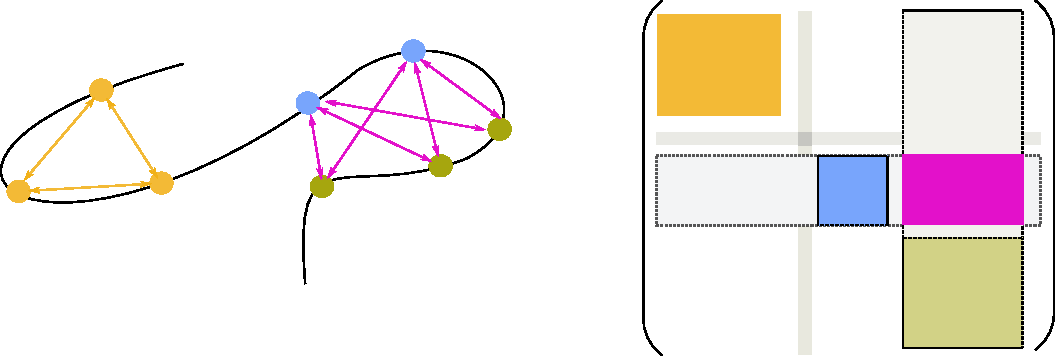
\includegraphics[trim=1cm 3cm 0cm 1cm, clip=true,scale=0.75]{figures/matrix} 
\caption{Energy matrix elements. {\bf For diagonal elements (above),} we show an example of an FDB element and an NEA element
  (one rotamer each). The individual energy components are labelled. ASA labels the surface energy term. Although the Arg1141
  position is treated with FDB, the matrix includes the NEA estimate of the GB contribution. The quantity labeled Q2 is the total
  squared charge $\sum_{i \in I} q_i^2$, needed to compute the solvation radius $B_I$ (Eq.\ \ref{eq:defB}). The five rightmost
  quantities are the fitting coefficients $c^{II}_n$ (Eq.\ \ref{eq:approx}). {\bf For off-diagonal elements (below),} we also
  show an FDB and an NEA pair (one rotamer combination each). For the FDB pair, the GB self-energy contributions $E_{IJ}^{\rm self}$
  and $E_{JI}^{\rm self}$ (Eq.\ \ref{eq:selfRR}) are both stored (the GB self energy is non-symmetric).} \label{fig:matrix}  
\end{figure}


\begin{figure}[h]
\centering
\includegraphics[trim=2cm 0cm 2cm 0cm, clip=true,scale=1.5]{figures/correlation_eps4} 
\caption{Comparison between computed and experimental \pk\ shifts.} \label{fig:correl}  
\end{figure}


\begin{figure}[h]
\centering
\includegraphics[trim=0cm 0cm 0cm 3.5cm, clip=true,scale=1.3]{figures/allOMTKexact} \\
\includegraphics[trim=0cm 0cm 0cm 0cm, clip=true,scale=1.3]{figures/coupling_eps4}
\caption{Above: OMTKY3 Titration curves. Below: titration of a coupled histidine pair in myoglobin (FDB results). The
pair binds one proton at low pH. ``MEAN'' indicates the mean number of protons per histidine (0.5 at low pH).} \label{fig:titrate}  
\end{figure}


\begin{figure}[h]
\centering
\includegraphics[trim=2.5cm 0cm 2cm 0cm, clip=true,scale=1.5]{figures/correlation_hemoglobin_eps4} 
\caption{Comparison between computed and experimental \pk\ shifts for hemoglobin.} \label{fig:hbcorrel}  
\end{figure}


\begin{figure}[h]
\centering
\includegraphics[trim=3cm 0cm 3cm 0cm, clip=true,scale=1.6]{figures/bohr_exp} \\
\caption{Bohr effect in hemoglobin due to histidine residues (excluding H45; see text). Both FDB and NEA predictions
  are shown. The separate contribution of $\beta$His146 is shown. } \label{fig:bohr}  
\end{figure}


\begin{figure}[!h]
\begin{center}
\vspace*{-1cm}
\includegraphics[trim=0cm 0cm 0cm 0cm, clip=true,scale=1.0]{figures/blosum.pdf}
\end{center}
\caption[width=1cm]{\small Histogram plots showing similarity scores for designed PDZ sequences. Similarity scores for the
entire protein (left) or 14 core positions (right). Values are shown for Proteus(NEA), Proteus(FDB), Rosetta, and Pfam sequences
(all compared to the Pfam RP55 alignment).} \label{fig:blosum}
\end{figure}

\end{document}
